\section{Exploración Univariada}\label{univariada}

En esta sección exploro cada índice. En esta sección exploro cada índice. En esta sección exploro cada índice. En esta sección exploro cada índice. En esta sección exploro cada índice. En esta sección exploro cada índice. En esta sección exploro cada índice. En esta sección exploro cada índice. En esta sección exploro cada índice.





Para conocer el comportamiento de las variables se ha preparado la Tabla \ref{Tfrecuencias}, donde se describe la distribución de las modalidades de cada variable. Los números representan la situación de algun país en ese indicador, donde el mayor valor numérico es la mejor situación.

% latex table generated in R 3.5.0 by xtable 1.8-2 package
% Fri Jun 29 16:07:02 2018
\begingroup\normalsize
\begin{longtable}{llrrr}
\caption{Tablas de Frecuencia de la variables en estudio} \\ 
 \textbf{Variable} & \textbf{Levels} & $\mathbf{n}$ & $\mathbf{\%}$ & $\mathbf{\sum \%}$ \\ 
  \hline \hline
WorldFreedom & 1 & 55 & 26.7 & 26.7 \\ 
   & 3 & 62 & 30.1 & 56.8 \\ 
   & 5 & 89 & 43.2 & 100.0 \\ 
   \hline
 & all & 206 & 100.0 &  \\ 
   \hline
\hline
EconomicFreedom & 1 & 21 & 10.1 & 10.1 \\ 
   & 2 & 78 & 37.7 & 47.8 \\ 
   & 3 & 74 & 35.8 & 83.6 \\ 
   & 4 & 28 & 13.5 & 97.1 \\ 
   & 5 & 6 & 2.9 & 100.0 \\ 
   \hline
 & all & 207 & 100.0 &  \\ 
   \hline
\hline
PressFreedom & 1 & 22 & 10.7 & 10.7 \\ 
   & 2 & 53 & 25.7 & 36.4 \\ 
   & 3 & 66 & 32.0 & 68.5 \\ 
   & 4 & 48 & 23.3 & 91.8 \\ 
   & 5 & 17 & 8.2 & 100.0 \\ 
   \hline
 & all & 206 & 100.0 &  \\ 
   \hline
\hline
Democracy & 1 & 60 & 29.1 & 29.1 \\ 
   & 2 & 45 & 21.8 & 51.0 \\ 
   & 4 & 82 & 39.8 & 90.8 \\ 
   & 5 & 19 & 9.2 & 100.0 \\ 
   \hline
 & all & 206 & 100.0 &  \\ 
   \hline
\hline
\hline
\label{Tfrecuencias}
\end{longtable}
\endgroup

Como apreciamos en la Tabla \ref{Tfrecuencias}, los países en la mejor situación son los menos, salvo en el caso del \emph{índice de libertas mundial}\footnote{Nótese que esto se puede deber a la {\bf menor} cantidad de categorías.}

\clearpage

Para resaltar lo anterior, tenemos la Figura \ref{barplots} en la página \pageref{barplots}. 


%%%%% figure
\begin{figure}[h]
\centering
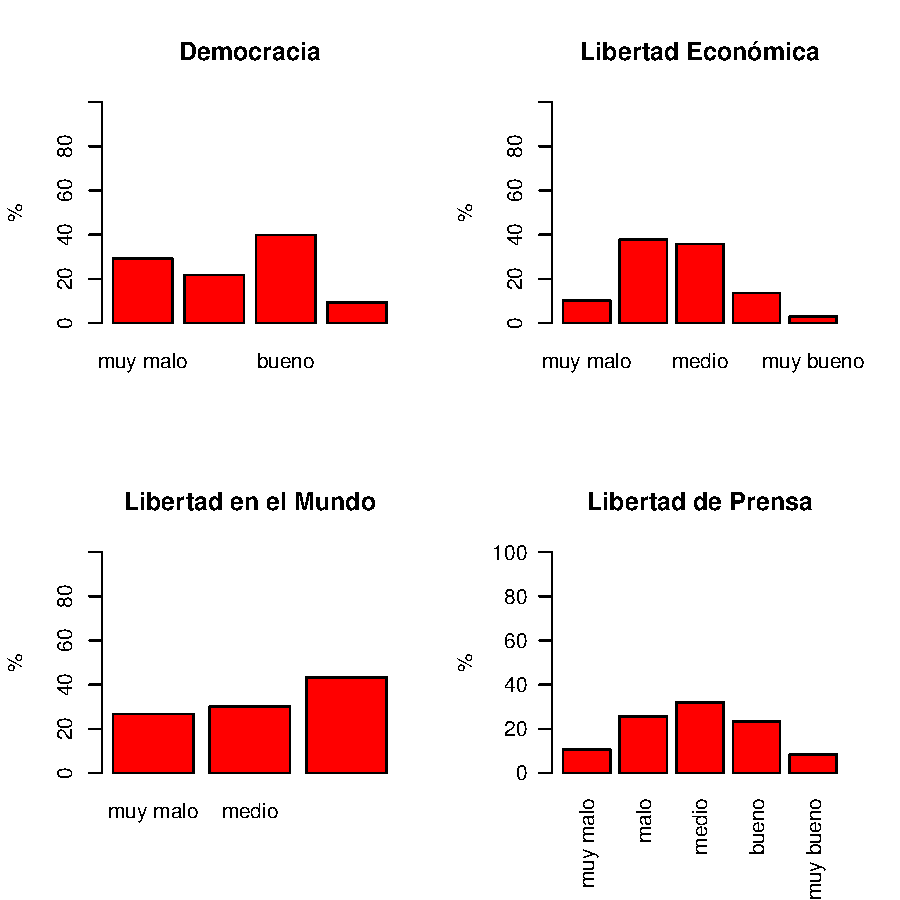
\includegraphics{paperVersion_7_univariada-barplots}
\caption{Distribución de Indicadores}
\label{barplots}
\end{figure}

Además de la distribución de los variable, es importante saber el valor central. Como los valores son de naturaleza ordinal debemos pedir la {\bf mediana} y otras medidas de posición (como los \emph{cuartiles}, los que no pediremos pues son pocos valores). La mediana de cada variable la mostramos en la Tabla \ref{stats} en la página \pageref{stats}.

% Table created by stargazer v.5.2.2 by Marek Hlavac, Harvard University. E-mail: hlavac at fas.harvard.edu
% Date and time: vie, jun 29, 2018 - 16:07:02
\begin{table}[!htbp] \centering 
  \caption{Medidas estadísticas} 
  \label{stats} 
\begin{tabular}{@{\extracolsep{5pt}}lcc} 
\\[-1.8ex]\hline 
\hline \\[-1.8ex] 
Statistic & \multicolumn{1}{c}{N} & \multicolumn{1}{c}{Median} \\ 
\hline \\[-1.8ex] 
WorldFreedom & 206 & 3.000 \\ 
EconomicFreedom & 207 & 3 \\ 
PressFreedom & 206 & 3.000 \\ 
Democracy & 206 & 2.000 \\ 
\hline \\[-1.8ex] 
\end{tabular} 
\end{table} 




\endinput
